\themaM
\graphicspath{{../../S07_Horaires_et_durees/Images/}}

\chapter{Horaires et durées}
\label{S07}


%%%%%%%%%%%%%%%%%%%%%%%%%%%%%%%%%%%%%%%%%%%
%\begin{prerequis}
%   \begin{itemize}
%      \item[\com] Mener des calculs impliquant des grandeurs mesurables.
%      \item[\com] Exprimer et vérifier la cohérence des résultats du point de vue des unités.
%      \item[\com] Effectuer des conversions d’unités.
%   \end{itemize}
%\end{prerequis}
%
%\vfill
%
%\begin{debat}[Débat : instruments anciens de mesure de temps et de durée]
%   De tous temps on a voulu mesurer le {\bf temps} et la {\bf durée}, ci-dessous figurent quelques instruments utilisés dans des époques plus ou moins lointaines. \\
%   \textcolor{B1}{\small
%   \begin{tabular}{*{4}{C{3.5}}}
%      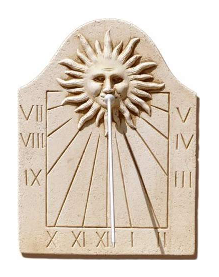
\includegraphics[width=2.8cm]{cadran}
%      &
%      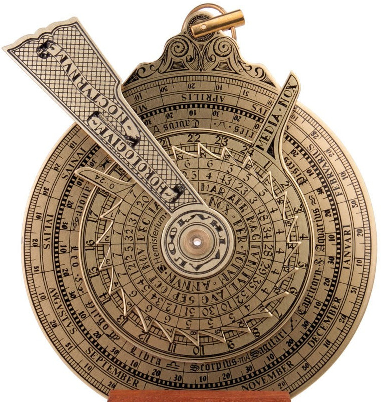
\includegraphics[width=2.8cm]{nocturlabe}
%      &
%      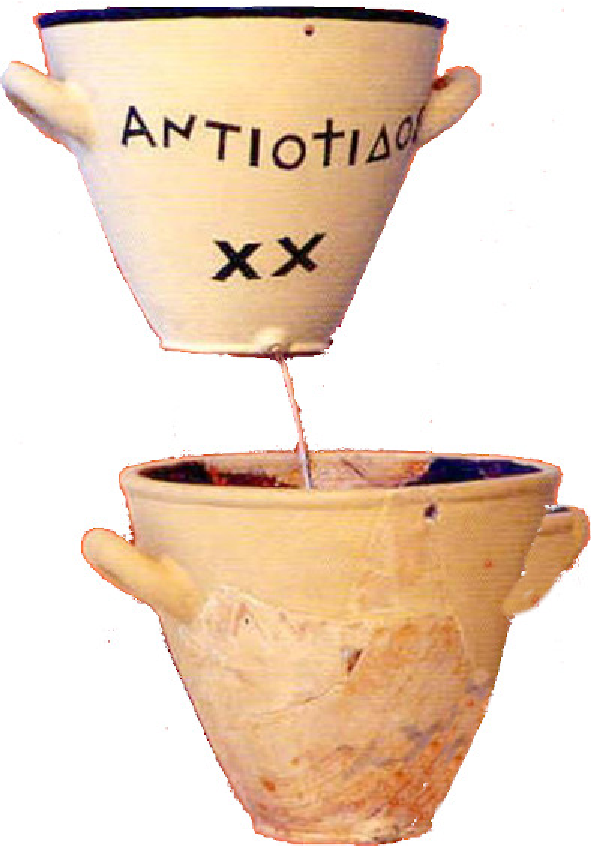
\includegraphics[width=2.8cm]{clepshydre}
%      &
%      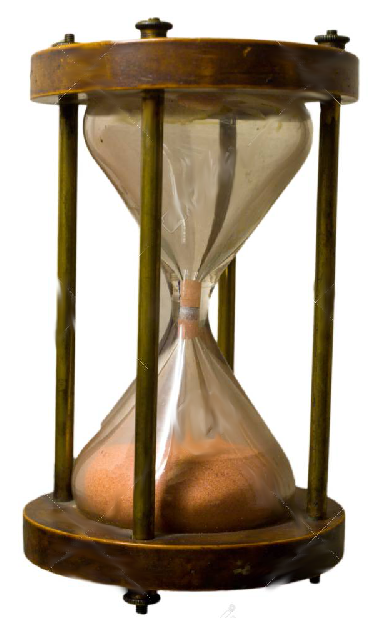
\includegraphics[width=2.8cm]{sablier} \\
%      Cadran solaire & Nocturlabe & Clepsydre & Sablier \\
%      1\,500 av. J.-C. & X\up{e} siècle & 1\,600 av. J.-C. & IX\up{e} siècle \\
%      Heures du jour & Heures de la nuit & Durées longues (heures) & Durées courtes (minutes) \\
%   \end{tabular}}
%   \bigskip
%   \begin{cadre}[B2][F4]
%      \begin{center}
%         Vidéo : \href{https://www.youtube.com/watch?v=8vMTE9U9z0U}{\bf Remettons les pendules à l'heure}, chaîne YouTube {\it C'est pas sorcier}.
%      \end{center}
%   \end{cadre}
%\end{debat}
%
%\vfill
%
%\textcolor{PartieGeometrie}{\sffamily\bfseries Cahier de compétences} : $\varnothing$
%
%
%%%%%%%%%%%%%%%%%%%%%%%%%%%%%%%%%%%%%%%%%%%%%%%%%%%%%%%%%%%%%%%%%%%%%%%
%\activites
% 
%\begin{activite}[De la seconde au siècle]
%   {\bf Objectif :} donner un ordre de grandeur dans le domaine des durées. \\
%   \begin{QCM}
%      Relier les durées suivantes à son ordre de grandeur.
%      \begin{center}
%         \begin{pspicture}(-8,-9)(8,9)
%         {\psset{yunit=0.85}
%            \rput(0,9){\large Siècle}
%            \rput(0,6){\large Année}
%            \rput(0,3){\large Mois}
%            \rput(0,0){\large Jour}
%            \rput(0,-3){\large Heure}
%            \rput(0,-6){\large Minute}
%            \rput(0,-9){\large Seconde}
%            \psdots(-1.5,-9)(-1.5,-6)(-1.5,-3)(-1.5,0)(-1.5,3)(-1.5,6)(-1.5,9)(1.5,-9)(1.5,-6)(1.5,-3)(1.5,0)(1.5,3)(1.5,6)(1.5,9)(-4,-10)(-4,-6)(-4,-2)(4,2)(4,6)(4,10)(4,-10)(4,-6)(4,-2)(-4,2)(-4,6)(-4,10)
%            \rput(-6.25,-6){\parbox{3.5cm}{Temps mis par la lumière pour parcourir une distance équivalente à celle séparant la Terre et la Lune}}
%            \rput(6.25,2){\parbox{3.5cm}{Durée d'un saison}}
%            \rput(-6.25,2){\parbox{3.5cm}{Record du monde du \um{100}}}
%            \rput(-6.25,-2){\parbox{3.5cm}{Temps de cuisson d'un \oe uf à la coque}}
%            \rput(6.25,6){\parbox{3.5cm}{Intervalle entre deux battements de c\oe ur consécutifs}}
%            \rput(-6.25,10){\parbox{3.5cm}{Durée d'un cycle complet de lune}}
%            \rput(6.25,-6){\parbox{3.5cm}{Durée d'un film}}
%            \rput(6.25,-10){\parbox{3.5cm}{Temps mis par la Terre pour faire le tour de son étoile : le Soleil}}
%            \rput(6.25,10){\parbox{3.5cm}{Âge maximum atteint par un humain}}
%            \rput(-6.25,6){\parbox{3.5cm}{Durée d'une grossesse}}
%            \rput(6.25,-2){\parbox{3.5cm}{Durée d'un entraînement de sport}}
%            \rput(-6.25,-10){\parbox{3.5cm}{Durée d'un weekend}}
%            \multido{\n=-9+3}{7}{\rput(0,\n){\psframe(-1,-0.5)(1,0.5)}}}
%         \end{pspicture}
%      \end{center}
%   \end{QCM}
%\end{activite}
%
%
%%%%%%%%%%%%%%%%%%%%%%%%%%%%%%%%%%
%%%%%%%%%%%%%%%%%%%%%%%%%%%%%%%%%%
%\cours 
%
%\section{Unités de temps} %%%
%
%Selon les situations, on indique les durées en années, mois, jours, heures, minutes, ou secondes : 1 siècle = 100 ans ; 1 an = 12 mois = 365 jours ou 366 jours ; 1 jour = 24 heures ; 1 heure = 60 minutes = 3\,600 secondes\dots \\
%Pour mesurer le temps ou une durée, on peut utiliser un cadran solaire, un sablier, une montre, un chronomètre\dots
%
%%%%%%%%%%%%%%%%%%%%%%%%%%%%%%%%%%%%
%\section{Conversion de durées}
%
%\begin{methode*2*2}
%   Pour convertir des heures en minutes ou des minutes en secondes ou inversement, on peut utiliser le schéma suivant : \\
%   \begin{pspicture}(-1,-2.5)(5,3)
%      \ovalnode{A}{durée en heures}
%      \ovalnode{B}{durée en minutes}
%      \ovalnode{C}{durée en secondes}
%      \nccurve[angle=90,linecolor=B1]{->}{A}{B}
%      \ncput*{\textcolor{B1}{$\times 60$}}
%      \nccurve[angle=90,linecolor=B1]{->}{B}{C}
%      \ncput*{\textcolor{B1}{$\times 60$}}
%      \nccurve[angle=-90,linecolor=A1]{->}{B}{A}
%      \ncput*{\textcolor{A1}{$\div 60$}}
%      \nccurve[angle=-90,linecolor=A1]{->}{C}{B}
%      \ncput*{\textcolor{A1}{$\div 60$}}
%      \nccurve[angle=90,linecolor=B1]{->}{A}{C}
%         \ncput*{\textcolor{B1}{$\times 3\,600$}}
%      \nccurve[angle=-90,linecolor=A1]{->}{A}{C}
%      \ncput*{\textcolor{A1}{$\div 3\,600$} }
%   \end{pspicture}
%   \exercice
%    Convertir 170 minutes en heures et minutes.     
%   \correction
%   $170=2\times60+50$, donc \\
%   $\umin{170} =\uh{2}\,\umin{50}$.
%   \exercice
%   Convertir \uh{1}\,\umin{25}\,\us{36} en secondes.
%   \correction
%   $\uh{1} =\us{3600}$ et $\umin{1} =\us{60}$ donc \\
%   $\uh{1}\,\umin{25}\,\us{36} =\us{3600}+25\times\us{60}+\us{36} =\us{5136}$.
%\end{methode*2*2}
%
%\ \\
%
%Pour effectuer des additions ou soustractions, on peut effectuer une opération experte (un peu périlleuse) ou procéder de proche en proche.
% 
%\begin{exemple}
%   \ \\ [-10mm]
%  \begin{itemize}
%      \item Un train part de Montpellier à \uh{8} 48. La durée du trajet pour se rendre à Paris est de \uh{3} et \umin{20}. \\
%      À quelle heure arrivera-t-il à Paris ? \\ [5mm]
%      \item Un automobiliste part de Montpellier à \uh{8} 35 et arrive à Perpignan à \uh{10} 20. \\
%   Quelle est la durée de son trajet ?
%   \end{itemize}
%\correction
%\ \\ [-10mm]
%   \begin{itemize}
%      \item   
%      \begin{tabular}{ccccc}
%         & 8 & h & 4 & 8 \\
%         $+$ & 3 & h & 2 & 0 \\
%         \hline
%         1 & $\cancel{1}$ & h & $\cancel{6}$ & 8 \\
%         \multicolumn{5}{c}{\psline{->}(0.5,0.3)(-0.5,-0.1)} \\
%         1 & 2 & h & 0 & 8 \\ [5mm]
%      \end{tabular}
%   \hspace{0.5cm}
%   \begin{tabular}{p{5cm}}
%      \small
%      on aligne les heures sous les heures, les minutes sous les minutes puis on additionne. Si le nombre de minutes est supérieur à 60, on soustrait \umin{60} et on ajoute \uh{1}.
%   \end{tabular} 
%   \item \uh{8}\,\umin{35} \quad $\xrightarrow{+\umin{25}}$ \quad \uh{9}\,\umin{00} \\
%   \uh{9}\,\umin{00} \quad $\xrightarrow{+\uh{1}}$ \quad \uh{10}\,\umin{00} \\
%   \uh{10}\,\umin{00}\quad $\xrightarrow{+\umin{20}}$ \quad \uh{10}\,\umin{20}. \\   
%   La durée totale du trajet est de \uh{1}\,\umin{45}.
%   \end{itemize}   
%\end{exemple}
%
%
%%%%%%%%%%%%%%%%%%%%%%%%%%%%%%%%%%%%%%%%%%%%%%%%%%%%%%%%%%%%%%%%%%%%%%%
%\exercicesbase
%
%\begin{colonne*exercice}
%
%\serie{Conversion de durées} %%%%%
%
%\bigskip
%
%\begin{exercice} %1
%   Convertir les durées données ci-dessous en heures et minutes.
%   \begin{enumerate}
%      \item \uh{1,5}.
%      \item \uh{2,25}.
%      \item \uh{0,3}.
%   \end{enumerate}
%\end{exercice}
%
%\begin{corrige}
%   \ \\ [-5mm]
%   \begin{enumerate}
%      \item $\uh{1,5} =\blue \uh{1}\,\umin{30}$.
%      \item $\uh{2,25} =\blue \uh{2}\,\umin{15}$.
%      \item $\uh{0,3} =0,3\times\umin{60} =\blue \umin{18}$.
%   \end{enumerate}
%\end{corrige}
%
%\bigskip
%
%
%\begin{exercice} %2
%   Convertir les durées données ci-dessous en heures décimales.
%   \begin{enumerate}
%      \item $\uh{6}\,\umin{30}$.
%      \item $\uh{2}\,\umin{45}$.
%      \item $\uh{8}\,\umin{33}$.
%   \end{enumerate}
%\end{exercice}
%
%\begin{corrige}
%   \ \\ [-5mm]
%   \begin{enumerate}
%      \item $\uh{6}\,\umin{30} =\blue \uh{6,5}$.
%      \item $\uh{2}\,\umin{45} =\blue \uh{2,75}$. \smallskip
%      \item $\uh{8}\,\umin{33} =\uh{8}+\dfrac{33}{60}\,\uh{} =\blue \uh{8,55}$.
%   \end{enumerate}
%\end{corrige}
%
%\bigskip
% 
% 
%\begin{exercice} %3
%   Convertir les durées données ci-dessous en minutes.
%   \begin{enumerate}
%      \item \uh{1}\,\umin{56}.
%      \item 2  j \umin{25}.
%      \item 1 j \uh{20}\,\umin{3}.
%   \end{enumerate}
%\end{exercice}
%
%\begin{corrige}
%   \ \\ [-5mm]
%   \begin{enumerate}
%      \item $\uh{1}\,\umin{56} =1\times\umin{60}+\umin{56} =\blue \umin{116}$.
%      \item $2\text{ j } \umin{25} =2\times24\times\umin{60}+\umin{25}$ \\
%         \quad $=\umin{2880}+\umin{25} =\blue \umin{2905}$.
%      \item $1\text{ j } \uh{20}\,\umin{3} =24\times\umin{60}+20\times\umin{60}+\small\umin{3}$ \\
%         \quad $=\umin{1440}+\umin{1200}+\umin{3} =\blue \umin{2643}$.
%   \end{enumerate}
%\end{corrige}
%
%
%\bigskip
%
%\begin{exercice} %4
%   Convertir les durées données ci-dessous en heures et minutes.
%   \begin{enumerate}
%      \item \umin{156}.
%      \item \umin{296}.
%      \item \umin{1603}.
%   \end{enumerate}
%\end{exercice}
%
%\begin{corrige}
%   \ \\ [-5mm]
%   \begin{enumerate}
%      \item $\umin{156} =2\times\umin{60}+\umin{36} =\blue \uh{2}\,\umin{36}$.
%      \item $\umin{296} =4\times\umin{60}+\umin{56} =\blue \uh{4}\,\umin{56}$.
%      \item $\umin{1603} =26\times\umin{60}+\umin{43}$ \\
%         \quad $=\uh{26}\,\umin{43} =\blue 1\text{ j}\,\uh{2}\,\umin{43}$.
%   \end{enumerate}
%\end{corrige}
%
%\bigskip
%
%
%\serie{Calcul de durées} %%%%%
%
%\bigskip
%
%\begin{exercice} %5
%   Effectuer les calculs suivants :
%   \begin{enumerate}
%      \item $\uh{3}\,\umin{45}+\uh{5}\,\umin{13}$
%      \item $\uh{5}\,\umin{38}+\uh{9}\,\umin{43}$
%      \item $\uh{11}\,\umin{28}-\uh{7}\,\umin{22}$
%      \item $\uh{15}\,\umin{35}-\uh{9}\,\umin{49}$
%   \end{enumerate}
%\end{exercice}
%
%\begin{corrige}
%   \ \\ [-5mm]
%   \begin{enumerate}
%      \item $\uh{3}+\uh{5} =\uh{8}$ et $\umin{45}+\umin{13} =\umin{58}$ donc, $\uh{3}\,\umin{45}+\uh{5}\,\umin{13} =\blue \uh{8}\,\umin{58}$.
%      \item $\uh{5}+\uh{9} =\uh{14}$ et \\
%         $\umin{38}+\umin{43} =\umin{81} =\uh{1}+\umin{21}$ \\
%         donc, $\uh{5}\,\umin{38}+\uh{9}\,\umin{43} =\blue \uh{15}\,\umin{21}$.
%      \item $\uh{7}\,\umin{22} \quad \xrightarrow{+\umin{38}} \quad \uh{8}\,\umin{00}$ \\
%         \quad\, $\uh{8}\,\umin{00} \quad \xrightarrow{+\uh{3}} \quad \uh{11}\,\umin{00}$ \\
%         \quad\, $\uh{11}\,\umin{00}\quad \xrightarrow{+\umin{28}} \quad \uh{11}\,\umin{28}$. \\   
%         $\uh{11}\,\umin{28}-\uh{7}\,\umin{22} =\uh{3}\,\umin{66} =\blue \uh{4}\,\umin{06}$.
%      \item $\uh{9}\,\umin{49} \quad \xrightarrow{+\umin{11}} \quad \uh{10}\,\umin{00}$ \\
%         \quad\, $\uh{10}\,\umin{00} \quad \xrightarrow{+\uh{5}} \quad \uh{15}\,\umin{00}$ \\
%         \quad\, $\uh{15}\,\umin{00}\quad \xrightarrow{+\umin{35}} \quad \uh{15}\,\umin{35}$. \\   
%         $\uh{15}\,\umin{35}-\uh{9}\,\umin{49} =\blue \uh{5}\,\umin{46}$.
%   \end{enumerate}
%\end{corrige}
%
%\bigskip
%
%
%\begin{exercice} %6
%   Hamza part à \uh{7}\,\umin{38} pour prendre le bus direction le collège Simone Veil. Il met 6 minutes pour aller jusqu'à l'arrêt de bus, puis le trajet en bus dure 16 minutes et enfin il lui reste 4 minutes à pied. \\
%   À quelle heure arrivera-t-il au collège ?
%\end{exercice}
%
%\begin{corrige}
%   Le temps de déplacement d'Hamza est de \\
%   $\umin{6}+\umin{16}+\umin{4} =\umin{26}$. \\
%   Or, $\uh{7}\,\umin{38}+\umin{26} =\uh{7}\,\umin{64} =\uh{8}\,\umin{04}$. \\
%   {\blue Hamza devrait arriver au collège à \uh{8}\,\umin{04}}. \\
%\end{corrige}
%
%\bigskip
%
%
%\begin{exercice} %7
%   Loane part du collège à pied à \uh{17}\,\umin{04}. Elle prévoit \umin{15}\,\us{30} pour le trajet, \umin{5} pour acheter un pain au chocolat et \umin{7} pour dire au revoir aux copines (et copains !). \\
%   À quelle heure arrivera-t-elle chez elle ?
%\end{exercice}
%
%\begin{corrige}
%   Le temps de déplacement de Loane est de \\
%   $\umin{15}\,\us{30}+\umin{5}+\umin{7} =\umin{27}\,\us{30}$. \\
%   Or, $\uh{17}\,\umin{04}+\umin{27}\,\us{30} =\uh{17}\,\umin{31}\,\us{30}$. \\
%   {\blue Loane devrait arriver chez elle à \uh{17}\,\umin{31}\,\us{30}}. \\
%\end{corrige}
%
%\bigskip
%
%
%\begin{exercice} %8
%   Duaa part en promenade à \uh{9} 20. Elle rentre à \uh{12}15, ne s'étant arrêté pour se reposer que lors de trois pauses de \umin{5} chacune. \\
%   Pendant combien de temps a-t-elle marché ?
%\end{exercice}
%
%\begin{corrige}
%   $\uh{9}\,\umin{20} \quad \xrightarrow{+\umin{40}} \quad \uh{10}\,\umin{00}$ \\
%   $\uh{10}\,\umin{00} \quad \xrightarrow{+\uh{2}} \quad \uh{12}\,\umin{00}$ \\
%   $\uh{12}\,\umin{00}\quad \xrightarrow{+\umin{15}} \quad \uh{12}\,\umin{15}$. \\   
%   La promenade de Duaa a duré \uh{2}\,\umin{55}. \\
%   Or, elle s'est arrêtée $3\times\umin{5} =\umin{15}$ donc, {\blue elle a marché durant \uh{2}\,\umin{40}}. \\
%\end{corrige}
%
%\bigskip
%
%
%\serie{Problèmes} %%%%%
%
%\bigskip
%
%\begin{exercice} %9
%   Dans une usine, une machine met \umin{5}\,\us{26} pour fabriquer une pièce.
%   \begin{enumerate}
%      \item Combien de temps met-elle pour fabriquer 5 pièces ?
%      \item Combien de temps met-elle pour en fabriquer 10 ?
%      \item Combien de temps met-elle pour en fabriquer 20 ?
%      \item Combien de temps met-elle pour en fabriquer 100 ?
%      \item Combien la machine aura-t-elle fabriqué de pièces si elle fonctionne \uh{8} sans s’arrêter ?
%      \item Une nouvelle machine, qui vient d’arriver à l’usine, met deux fois moins de temps pour fabriquer la même pièce. \\
%      Quel temps met-elle pour fabriquer la pièce ?
%   \end{enumerate}
%\end{exercice}
%
%\begin{corrige}
%   \ \\ [-5mm]
%   \begin{enumerate}
%      \item Pour 5 pièces : \\
%         $5\times\umin{5} =\umin{25} ; 5\times\us{26} =\us{130} =\umin{2}\,\us{10}$. \\
%         $\umin{25}+\umin{2}\,\us{10} =\blue \umin{27}\,\us{10}$.
%      \item Pour 10 pièces, c'est-à-dire 2 fois 5 pièces : \\
%         $2\times(\umin{27}\,\us{10}) =\blue \umin{54}\,\us{20}$.
%      \item Pour 20 pièces, c'est à dire 2 fois 10 pièces : \\         $2\times(\umin{54}\,\us{20}) =\umin{108}\,\us{40} =\blue \uh{1}\,\umin{48}\,\us{40}$.
%      \item Pour 100 pièces, c'est à dire 10 fois 10 pièces : \\
%         $10\times(\umin{54}\,\us{20}) =\umin{540}\,\us{200} =\blue \uh{9}\,\umin{3}\,\us{20}$.
%      \item $\uh{8} =8\times\us{3600} =\us{28800}$ et \\
%         $\umin{5}\,\us{26} =5\times\us{60}+\us{26} =\us{326}$. \\
%      Or, $28\,800\div326 \approx88,34$ donc, {\blue la machine aura fabriqué 88 pièces en \uh{8}}.
%      \item La moitié de \umin{5} vaut \umin{2}\,\us{30} et la moitié de \us{26} vaut \us{13} donc, {\blue la machine met \umin{2}\,\us{43}}.
%   \end{enumerate}
%\end{corrige}
%
%\bigskip
%
%
%\begin{exercice} %10
%   On voit un éclair quasiment à l’instant où il se produit (la lumière a une vitesse de \ukms{300 000}), mais le bruit (coup de tonnerre) n’est entendu qu’un peu plus tard car la vitesse du son est d’environ \ums{340}, soit à peu près 1 million de fois plus lent.
%   \begin{enumerate}
%      \item Concrètement, que veut dire le fait que la lumière a une vitesse de \ukms{300 000} ?
%      \item Si on entend le tonnerre 6 secondes après avoir vu l'éclair, à quelle distance se situe l'orage ?
%      \item Erdogan se trouve à \ukm{8,5} d'une orage. il voit un éclair. Combien de temps se passera-t-il avant qu'il n'entende le tonnerre ?
%      \item Justifier la technique qui consiste à compter les secondes entre l'éclair et le tonnerre et à les diviser par 3 pour obtenir la distance (en kilomètre) à laquelle la foudre est tombée.
%   \end{enumerate}
%\end{exercice}
%
%\begin{corrige}
%   \ \\ [-5mm]
%   \begin{enumerate}
%      \item Une vitesse de \ukmh{300 000} signifie que {\blue la lumière parcourt \ukm{300000} en une heure}.
%      \item Le son parcourt \um{340} en une seconde, soit $6\times\um{340} =\um{2040}$ en 6 secondes. \\
%         {\blue L'orage se situe à environ \ukm{2}}.
%      \item $\ukm{8,5} =\um{8500}$. or, $\um{8500}\div\um{340} =25$ donc,  {\blue Erdogan entendra le tonnerre 25 secondes après l'avoir vu}.
%      \item Le tonnerre met une seconde pour parcourir la distance de \um{340}, soit 3 secondes pour parcourir $3\times\um{340} =\um{1020} =\ukm{1,02}$. Cela signifie qu'à chaque fois que l'on compte 3 secondes, le son a parcouru \ukm{1}. C'est pourquoi {\blue il suffit de diviser le nombre de secondes par 3 pour obtenir la distance de l'orage}.
%   \end{enumerate}
%   
%\Coupe
%
%\corec{Quel degré est-il ?}
%
%\begin{enumerate}
%   \item Lorsqu'une aiguille parcourt la totalité du cadran, elle parcourt 360\degre. Donc, l'écart entre deux graduations des heures vaut 30\degre{} ($360\div12 =30$) et l'écart entre deux graduations des minutes vaut 6\degre{} ($360\div60 =6$).
%   \begin{itemize}
%      \item Il est 8 h\dots \\
%         {\psset{unit=0.7}
%          \begin{pspicture}(-5,-2.2)(2.5,2.2)
%             \pscircle[linewidth=1mm](0,0){2}
%             \multido{\i=0+6}{60}{\psline[linecolor=A1](1.8;\i)(2;\i)} %minutes
%             \multido{\i=0+30}{12}{\psline[linecolor=B2](1.7;\i)(2;\i)} %heures             
%             \multido{\i=60+-30,\n=1+1}{12}{\rput(1.5;\i){\scriptsize\n}} %écritures
%             \psline[linewidth=1mm,linecolor=B2]{->}(0,0)(1;-150)
%             \psline[linewidth=1mm,linecolor=A1]{->}(0,0)(1.3;90)
%             \psdot(0,0)
%             \psarc[linecolor=J1]{<->} (0,0){1}{90}{-150}
%            \rput(-0.5,0.25){\textcolor{J1}{\scriptsize 120\degre}}
%         \end{pspicture}} \\
%         À 8 h 00, la grande aiguille est sur le 12 et la petite aiguille est sur le 8. \\
%         Il y a donc 4 graduations des heures entre les deux. \\
%         Or, $4\times 30^\circ =120^\circ$. Donc, {\blue l'angle formé par les deux aiguilles lorsqu'il est 8 h 00 est de 120\degre}.
%         \item Il est 10 h 30\dots \\
%         {\psset{unit=0.7}
%         \begin{pspicture}(-5,-2.2)(2.5,2.2)
%            \pscircle[linewidth=1mm](0,0){2}
%            \multido{\i=0+6}{60}{\psline[linecolor=A1](1.8;\i)(2;\i)} %minutes
%            \multido{\i=0+30}{12}{\psline[linecolor=B2](1.7;\i)(2;\i)} %heures             
%            \multido{\i=60+-30,\n=1+1}{12}{\rput(1.5;\i){\scriptsize\n}} %écritures
%            \psline[linewidth=1mm,linecolor=B2]{->}(0,0)(1;135)
%            \psline[linewidth=1mm,linecolor=A1]{->}(0,0)(1.3;-90)
%            \psdot(0,0)
%            \psarc[linecolor=J1]{<->} (0,0){1}{135}{-90}
%            \rput(-0.5,-0.25){\textcolor{J1}{\scriptsize 135\degre}}
%          \end{pspicture}} \\
%            À 10 h 30, la grande aiguille est sur le 6 et la petite aiguille est juste entre le 10 et le 11, il y a donc 4,5 graduations des heures entre les deux. \\
%            Or, $4,5\times30^\circ =135^\circ$. Donc, {\blue l'angle formé par les deux aiguilles lorsqu'il est 10 h 30 est de 135\degre}.
%         \item Il est 6h 20\dots \\
%         {\psset{unit=0.7}
%         \begin{pspicture}(-5,-2.2)(2.5,2.2)
%            \pscircle[linewidth=1mm](0,0){2}
%            \multido{\i=0+6}{60}{\psline[linecolor=A1](1.8;\i)(2;\i)} %minutes
%            \multido{\i=0+30}{12}{\psline[linecolor=B2](1.7;\i)(2;\i)} %heures             
%            \multido{\i=60+-30,\n=1+1}{12}{\rput(1.5;\i){\scriptsize\n}} %écritures
%            \psline[linewidth=1mm,linecolor=B2]{->}(0,0)(1;-100)
%            \psline[linewidth=1mm,linecolor=A1]{->}(0,0)(1.3;-30)
%            \psdot(0,0)
%            \psarc[linecolor=J1]{<->} (0,0){1}{-100}{-30}
%            \rput(0.35,-0.55){\textcolor{J1}{\scriptsize 70\degre}}
%         \end{pspicture}} \\
%         À 6 h 20, la grande aiguille est sur le 4 et la petite aiguille est entre le 6 et le 7, à un tiers du 6, il y a donc 2 graduations des heures plus un tiers entre les deux. \\
%            Or, $2\times30^\circ+1\div3\times 30^\circ =60^\circ+10^\circ =70^\circ$. \\
%            Donc, {\blue l'angle formé par les deux aiguilles lorsqu'il est 6 h 20 est de 70\degre}.      
%      \end{itemize}
%   \end{enumerate}
%   
%\Coupe
%
%   \begin{enumerate}
%   \setcounter{enumi}{1}
%      \item À chaque fois que l'aiguille des minutes parcourt 5 minutes (30\degre), l'aiguille des heures parcourt 2,5\degre ($30\div12 =2,5$). \\
%      On choisit alors l'angle le plus petit entre les deux aiguilles et dans le tableau suivant, on indique l'angle le plus petit des aiguilles avec le \og 12 \fg. \\ [2mm]
%      {\hautab{1.5}
%      \begin{Ltableau}{0.9\linewidth}{4}{c}
%         \hline
%         heure & aiguille des minutes & aiguille des heures & angle entre les deux \\
%         \hline
%         0 h 00 & 0\degre & 0\degre & 0\degre \\
%         0 h 05 & 30\degre & 2,5\degre & 27,5\degre \\
%         0 h 10 & 60\degre & 5\degre & 55\degre \\
%         0 h 15 & 90\degre & 7,5\degre & 82,5\degre \\
%         0 h 20 & 120\degre & 10\degre & 110\degre \\
%         0 h 25 & 150\degre & 12,5\degre & 137,5\degre \\
%         0 h 30 & 180\degre & 15\degre & 165\degre \\
%         0 h 35 & 150\degre & 17,5\degre & 167,5\degre \\
%         0 h 40 & 120\degre & 20\degre & \textcolor{blue}{140\degre} \\
%         \hline
%      \end{Ltableau}}
%   {\blue Il est minuit et 40 minutes}.
%   \end{enumerate}
%
%\end{corrige}
%
%\end{colonne*exercice}
%
%
%%%%%%%%%%%%%%%%%%%%%%%%%%%%%%%%%%%%%%%%%%%
%\Recreation
%
%\enigme[quel degré est-il ?]
%   À une heure donnée, on fait correspondre l'angle le plus petit formé par les deux aiguilles, par exemple : \\
%   \begin{minipage}{4cm}
%      \uh{15}\,00 correspond à \udeg{90}
%   \end{minipage}
%   \begin{minipage}{8cm}
%      {\psset{unit=0.7}
%      \begin{pspicture}(-2.5,-2.5)(2.5, 2.5)
%         \pscircle[linewidth=1mm](0,0){2}
%         \multido{\i=0+6}{60}{\psline[linecolor=A1](1.8;\i)(2;\i)} %minutes
%         \multido{\i=0+30}{12}{\psline[linecolor=B2](1.7;\i)(2;\i)} %heures             
%         \multido{\i=60+-30,\n=1+1}{12}{\rput(1.5;\i){\scriptsize\n}} %écritures
%         \psline[linewidth=1mm,linecolor=B2]{->}(0,0)(1;0)
%         \psline[linewidth=1mm,linecolor=A1]{->}(0,0)(1.3;90)
%         \psdot(0,0)
%         \psarc[linecolor=gray]{<->} (0,0){1}{0}{90}
%         \rput(0.5,0.5){\textcolor{gray}{\scriptsize 90\degre}}
%      \end{pspicture}
%      \qquad 
%      \begin{pspicture}(-2.5,-2.5)(2.5,2.5)
%         \pscircle[linewidth=1mm](0,0){2}
%         \multido{\i=0+6}{60}{\psline[linecolor=A1](1.8;\i)(2;\i)} %minutes
%         \multido{\i=0+30}{12}{\psline[linecolor=B2](1.7;\i)(2;\i)} %heures             
%         \multido{\i=60+-30,\n=1+1}{12}{\rput(1.5;\i){\scriptsize\n}} %écritures
%         \psline[linewidth=1mm,linecolor=B2]{->}(0,0)(1;-90)
%         \psline[linewidth=1mm,linecolor=A1]{->}(0,0)(1.3;90)
%         \psdot(0,0)
%         \psarc[linecolor=gray]{<->} (0,0){1}{-90}{90}
%         \rput(0.5,0){\textcolor{gray}{\scriptsize 180\degre}}
%      \end{pspicture}}
%      \end{minipage}
%      \begin{minipage}{4cm}
%         \uh{18} correspond à \udeg{180}
%      \end{minipage}
%   \begin{enumerate}
%      \item Indiquer, en justifiant, l'angle correspondant à chacune des heures suivantes : \\
%      \begin{center}
%         {\psset{unit=0.7}
%         \begin{tabular}{C{4}|C{6}|C{4}}
%            \uh{8} & \uh{10}\,30 & \uh{6}\,20 \\
%            \begin{pspicture}(-2.5,-2.5)(2.5,2.5)
%               \pscircle[linewidth=1mm](0,0){2}
%               \multido{\i=0+6}{60}{\psline[linecolor=A1](1.8;\i)(2;\i)} 
%               \multido{\i=0+30}{12}{\psline[linecolor=B2](1.7;\i)(2;\i)}             
%               \multido{\i=60+-30,\n=1+1}{12}{\rput(1.5;\i){\scriptsize\n}}
%               \psdot(0,0)
%            \end{pspicture}
%            &
%            \begin{pspicture}(-2.5,-2.5)(2.5,2.5)
%               \pscircle[linewidth=1mm](0,0){2}
%               \multido{\i=0+6}{60}{\psline[linecolor=A1](1.8;\i)(2;\i)} 
%               \multido{\i=0+30}{12}{\psline[linecolor=B2](1.7;\i)(2;\i)}             
%               \multido{\i=60+-30,\n=1+1}{12}{\rput(1.5;\i){\scriptsize\n}}
%               \psdot(0,0)
%            \end{pspicture}
%            &
%            \begin{pspicture}(-2.5,-2.5)(2.5,2.5)
%               \pscircle[linewidth=1mm](0,0){2}
%               \multido{\i=0+6}{60}{\psline[linecolor=A1](1.8;\i)(2;\i)}
%               \multido{\i=0+30}{12}{\psline[linecolor=B2](1.7;\i)(2;\i)}             
%               \multido{\i=60+-30,\n=1+1}{12}{\rput(1.5;\i){\scriptsize\n}}
%               \psdot(0,0)
%            \end{pspicture} \\ [40mm]
%         \end{tabular}}
%      \end{center}
%      \ \\
%      \item Il est entre minuit et une heure du matin, l'aiguille des minutes est sur une des douze graduations du cadran, les deux aiguilles forment un angle de \udeg{140}. Quelle heure est-il ? \\
%      {\psset{unit=1.4}
%      \begin{pspicture}(-2.5,-2.5)(2.5,2.5)
%         \pscircle[linewidth=1mm](0,0){2}
%         \multido{\i=0+6}{60}{\psline[linecolor=A1](1.8;\i)(2;\i)} %minutes
%         \multido{\i=0+30}{12}{\psline[linecolor=B2](1.7;\i)(2;\i)} %heures             
%         \multido{\i=60+-30,\n=1+1}{12}{\rput(1.5;\i){\small\n}} %écritures
%         \psdot(0,0)
%      \end{pspicture}}
%   \end{enumerate}
%
